\documentclass{anstrans}
%%%%%%%%%%%%%%%%%%%%%%%%%%%%%%%%%%%
\title{}
\author{Baptiste Mouginot,$^{*}$ Kathryn Mummah,$^{*}$ Paul P.H.  Wilson$^{*}$}

\institute{
$^{*}$University of Wisconsin-Madison, WI
}

\email{mouginot@wisc.edu \and mummah@wisc.edu \and paul.wilson@wisc.edu}

% Optional disclaimer: remove this command to hide
% \disclaimer{Notice: this manuscript is a work of fiction.  Any resemblance to
% actual articles, living or dead, is purely coincidental.}

%%%% packages and definitions (optional)
\usepackage{graphicx} % allows inclusion of graphics
\usepackage{booktabs} % nice rules (thick lines) for tables
\usepackage{microtype} % improves typography for PDF
\usepackage{float}

\newcommand{\SN}{S$_N$}
\renewcommand{\vec}[1]{\bm{#1}} %vector is bold italic
\newcommand{\vd}{\bm{\cdot}} % slightly bold vector dot
\newcommand{\grad}{\vec{\nabla}} % gradient
\newcommand{\ud}{\mathop{}\!\mathrm{d}} % upright derivative symbol


\usepackage[acronym]{glossaries}
\newacronym{UOX}{UOX}{uranium oxide fuel}
\newacronym{MOX}{MOX}{mixed oxide fuel}
\newacronym{LWR}{LWR}{light water reactor}
\newacronym{FBR}{FBR}{fast breeder reactor}

\begin{document}
%%%%%%%%%%%%%%%%%%%%%%%%%%%%%%%%%%%%%%%%%%%%%%%%%%%%%%%%%%%%%%%%%%%%%%%%%%%%%%%%
\section{Introduction}

Fuel cycle simulations, as any simulation process, do not produce results
without errors.  Those errors have different sources: data uncertainties (when
the simulation relies on previously estimated/measured metrics), modeling
uncertainties (produced by the simplification made by the simulator) and the
``operational`` uncertainty (uncertainty on the operation parameters of the
different facilities).

Some treaty verification scenarios require estimating historical fissile
material production based on records of facility operation and material
transfer.  If the measurements of facility operation and material transfer are
subject to uncertainty, the total production quantities will then also be
uncertain, creating an opportunity for undetected diversion.  This study seeks
to understand which measures of facility operation have the most impact on the
uncertainty of fissile material production across a complete fuel cycle.  An
approaching using Total Monte Carlo methodology will be applied to the Cyclus
fuel cycle simulator \cite{cyclus} to estimate output metrics uncertainty caused
by individual facility uncertainties.

% I don't think Total Monte Carlo should be in quotes
\section{The Experiment}

\subsection{Method}

To estimate the uncertainty on fuel cycle output metrics, a Total Monte
Carlo approach has been applied.  In the following, output metric uncertainty
corresponds to the Standard Deviation of the output metrics over about 200
different simulations.  For each deployed facilities, the uncertainty associated
parameters have been a normally distributed with an artificially large standard
deviation of $10\%$.

To pursuit this work, both the Cycamore\cite{cycamore} package\footnote{Low
fidelity facilities package for Cyclus} and the
CyCLASS\footnote{Reactor and Fuel fabrication facility based on
    CLASS\cite{CLASS}  models} have been
updated\cite{mouginot_2018, cyclass} to deal with uncertainty in several
operational parameters of their associated facilities.  Table
\ref{tab:package_uncertainty} summarizes all modification implemented in the
range of facilities present in Cycamore and CyCLASS.


\begin{table}[htb]
\centering
  \caption{Summary of facility modification per source package.}
\begin{tabular}{cll}
\toprule

Package   & Facility   & Parameters                \\
\midrule
Cycamore & Separation & Separation efficiency     \\
         & Storage    & Residence Time            \\
\midrule
CyCLASS  & Reactor    & Cycle Length              \\
         &            & Power                     \\
         &            & Fuel Enrichment (PWR-UOX) \\

\bottomrule
\end{tabular}

  \label{tab:package_uncertainty}
\end{table}

The uncertainty on the different parameters have been considered for this study
as systematic for each new deployed facilities: each time a new facility is
deployed (such as a reactor or a fuel fabrication facility) a new set a
parameter is computed.

It must be noted that for this work, the fuel enrichment was determined by a
fuel fabrication model\cite{Leniau2015125} which
calculates the fissile fraction required in the fuel to reach a target
burnup at the end of irradiation.  In this study, the uncertainty on the fuel
enrichment is not applied directly on the effective enrichment but on the target
parameter (the burnup), which leads to a fuel enrichment uncertainty close to
$10\%$.

\subsection{The Fuel Cycle}
This work aims to assess the impact of the operational uncertainties of a simple
transition as shown in Figure \ref{fig:cycle}, inspired from the EG23 fuel cycle
of the Nuclear Fuel Cycle Evaluation and Screening Report\cite{ES}: a
transition from light water reactors fleet loaded with \glspl{UOX} fuel to a
sodium fast reactor fleet loaded \glspl{MOX} fuel, considering an $1\%/$y growth
of the generated power (Figure \ref{fig:power}).
\begin{figure}[ht] % replace 't' with 'b' to force it to be on the bottom
  \centering
  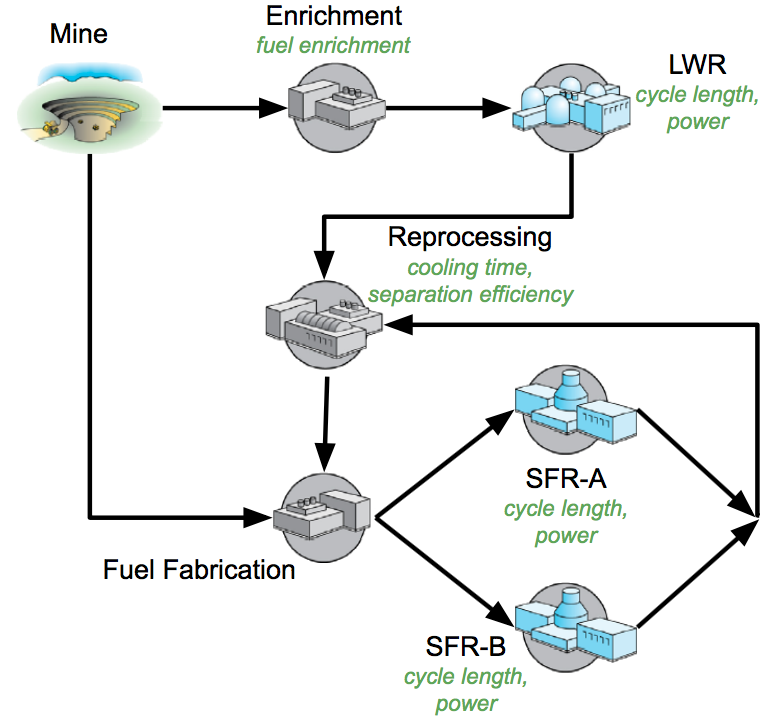
\includegraphics[scale=0.31]{cycle.png}
  \caption{Illustration of the material flow between the different facilities,
  with in green each operational parameters associated with an
  uncertainty.}\label{fig:cycle}
\end{figure}

As illustrated in Figure \ref{fig:power}, the transition starts with a fleet
fully composed of \glspl{LWR} loaded with enriched \glspl{UOX} fuel.  The actual
transition starts around year 35, with the deployment of \glspl{FBR}, loaded
with \glspl{MOX}, consisting of plutonium blended with natural
uranium.

\begin{figure}[ht] % replace 't' with 'b' to force it to be on the bottom
    \centering
    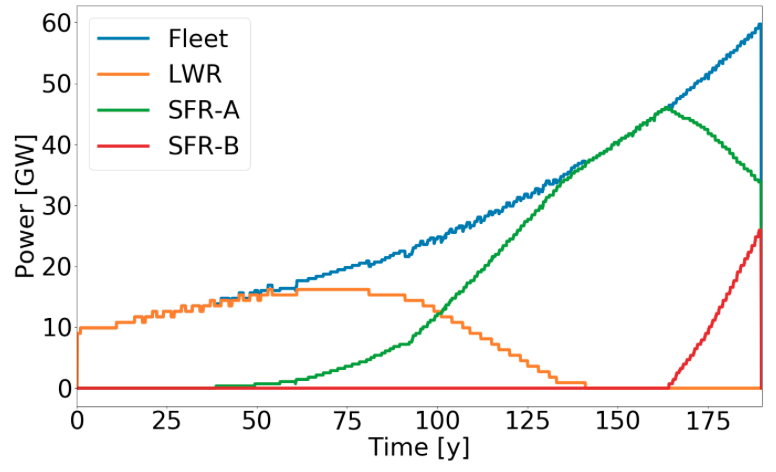
\includegraphics[scale=0.18]{power.png}
    \caption{Electric power generated over time, with in blue the full production,
        in orange the \glspl{LWR} contribution, in green the \glspl{FBR}.}
    \label{fig:power}
\end{figure}


The plutonium, required for \glspl{MOX} fabrication, is reprocessed from all
used fuel.  At first , it is sourced only from UOX, then used MOX fuel as it becomes
available for reprocessing.

Both fuel reprocessing and fabrication are done at a constant rate (constrained
by the feed materials availabilities).  The enrichment of the UOX is processed on
demand.  Buffer storages (not shown on Figure \ref{fig:cycle}) is present between
all facilities with constant processing rates.

In this works, a time step of 1 month have been considered.

\section{Results}

As nuclear archaeology main interests are high enrich uranium production and
fissile inventories, this specific study will mainly focus on the uncertainty on
the total quantity of natural uranium used and on the total unused fissile
inventory (unused reprocessed plutonium).  

Generated power will briefly being investigated to ensure the overall
uncertainty study will not be contaminated with fuel miss loading, which could
be interesting but are not the focus on this work.

For this study 6 set of 199 simulations, and a reference calculation have been
computed: One for each of the 5 uncertain parameters, one varying parameter the
4 others remaining fix, one with all 5 parameters varying and one single
simulation where all the 5 parameters were fixed at the mean value. 

In the following, each total uncertainty is reported at $\pm1\sigma$ around the
mean values of the corresponding uncertainty set at each time step. The time
dependant relative uncertainty are computed as the standard deviation of a
single set over its mean value at the corresponding time.


\subsection{Generated Power}

By construction, the very low uncertainty (Figure \ref{fig:power_full}) on the
generated power is expected.

\begin{figure}[h!] % replace 't' with 'b' to force it to be on the bottom
    \centering
    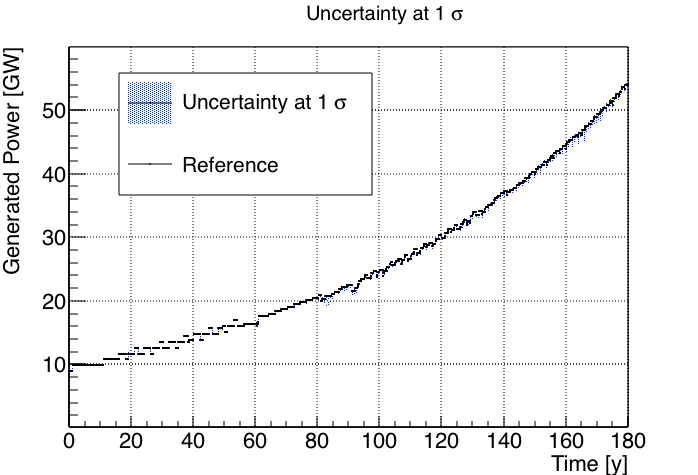
\includegraphics[scale=0.35]{power_full}
    \caption{Electric power generated as a function of time.  The black line
        represents the reference calculation and the blue zone
        represents the 1 $\sigma$ uncertainty distribution.}\label{fig:power_full}
\end{figure}

Indeed the transition scenario has been design to allow all the reactors to
receive the fuel as needed allowing them to be producing power all the time.
This ensures that the uncertainty measured any other parameters is not
influenced by the reactors miss-loadings.

%%  \begin{figure}[ht] % replace 't' with 'b' to force it to be on the bottom
%%    \centering
%%    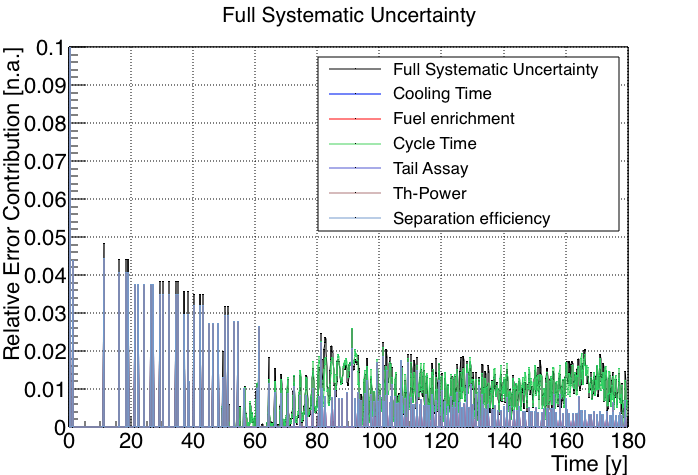
\includegraphics[scale=0.37]{power_uncer}
%%    \caption{}\label{fig:power_uncer}
%%  \end{figure}

\subsection{Natural Uranium Consumption dedicated to PWR-UOX fabrication}

Figure \ref{fig:unat_full} represents the cumulative natural uranium consumption
dedicated to PWR-UOX fuel fabrication as a function of time.  The uncertainty on
the cumulative uranium consumption grows as expected with the time and the
loading of the \glspl{LWR}.  The increase stops around year 125y with the
decommissioning of the last \glspl{LWR}.

\begin{figure}[ht] % replace 't' with 'b' to force it to be on the bottom
    \centering
    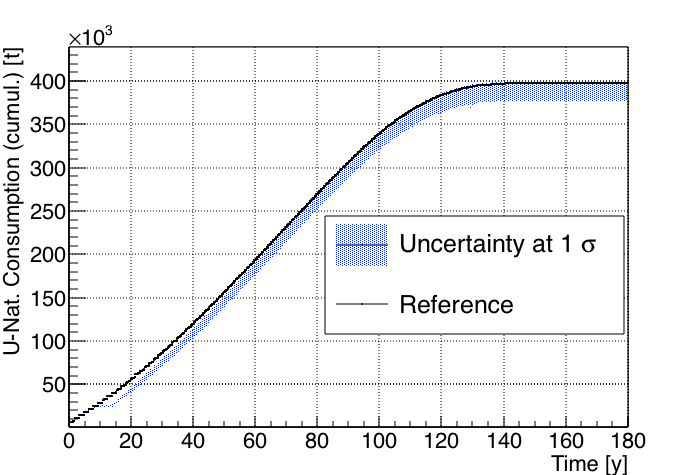
\includegraphics[scale=0.35]{unat_full}
    \caption{Cumulative consumption of natural uranium as a function of time.  The black line
        represents the reference calculation and the blue zone
        represents the 1 $\sigma$ uncertainty distribution.}\label{fig:unat_full}
\end{figure}


The fluctuation of the full relative uncertainty at low time are induced by the
fuel loading: all reactors at the beginning of the simulation have synchronised
cycle, this phenomenon disappears with the gradual decommissioning of the
initial reactors, spread on 50 years.


\begin{figure}[h!!] % replace 't' with 'b' to force it to be on the bottom
    \centering
    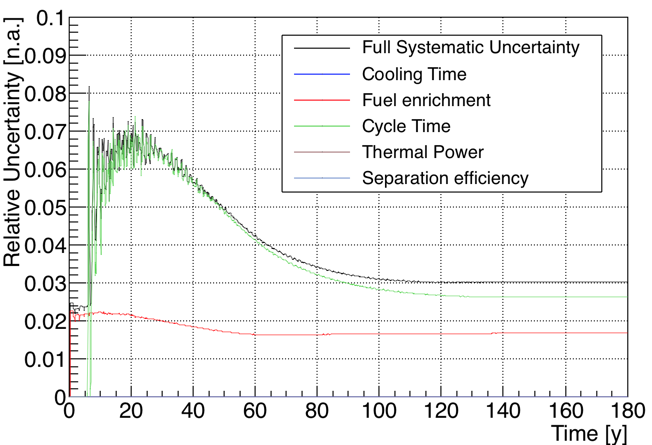
\includegraphics[scale=0.35]{unat_uncer}
    \caption{Cumulative natural uranium consumption relative uncertainty, with
    in black the total uncertainty at 1$\sigma$, and in color the uncertainty
    contribution of each parameter: cooling time (blue), fuel enrichment (red),
    cycle time (green), thermal power(brown), separation efficiency (light
    blue).}\label{fig:unatr_uncer}
\end{figure}
The relative uncertainty of the total uranium consumption starts at about
$5.5\%$ a slowly drops and stabilise around $3\%$.

As expected, cooling time, separation efficiency and thermal power don't
affect the natural uranium consumption.  The uncertainty on the natural uranium
consumption is dominated by the \glspl{LWR} cycle length: shorter the cycle
length is, the more fuel will be loaded.

With the increase of deployed reactors, the number of batches of \glspl{LWR}
fuel loaded converges to the references one (a random cycle length
values if randomly determined for each deployed reactors), reducing its impact
on the uncertainty on the total uranium consumption.
The fuel enrichment contribution follow a close to constant uncertainty
contribution of $2\%$, so as the total relative uncertainty decrease, its
relative contribution increases over time.

\subsection{Fissile Inventory}
The fissile inventory corresponds to the amount on separated fissile waiting to
be blend with natural uranium in order to produce the \glspl{FBR} MOX fuel.

As observed on Figure \ref{fig:pu_full}, the fissile inventory starts to grow on
year 40, with the deployment of the first reprocessing facility.  It grows
during the first period of the \glspl{LWR} to \glspl{FBR}-A transition until
year 90, then decrease slightly as the last \glspl{LWR} are decommissioned.
When he steady state is reached (full \glspl{FBR} fleet), the plutonium
inventory starts to increase, as the breading ratio of the \glspl{FBR} is higher
than the deployment needs.

\begin{figure}[ht] % replace 't' with 'b' to force it to be on the bottom
    \centering
    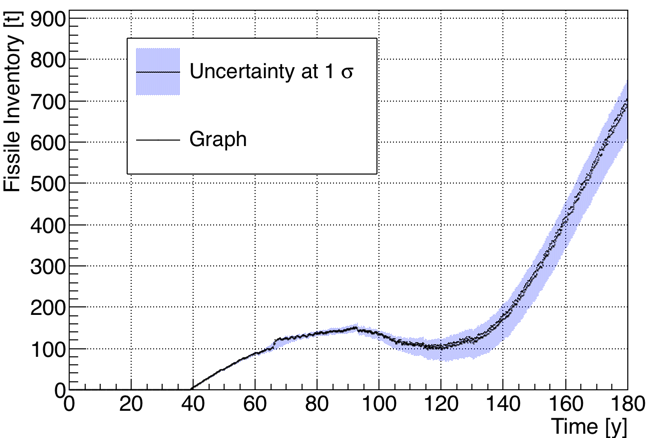
\includegraphics[scale=0.35]{pu_full}
    \caption{Fissile (plutonium) inventory as a function of time.  The black line
        represents the reference calculation and the blue zone
        represents the 1 $\sigma$ uncertainty distribution.}\label{fig:pu_full}
\end{figure}

\begin{figure}[h!!] % replace 't' with 'b' to force it to be on the bottom
    \centering
    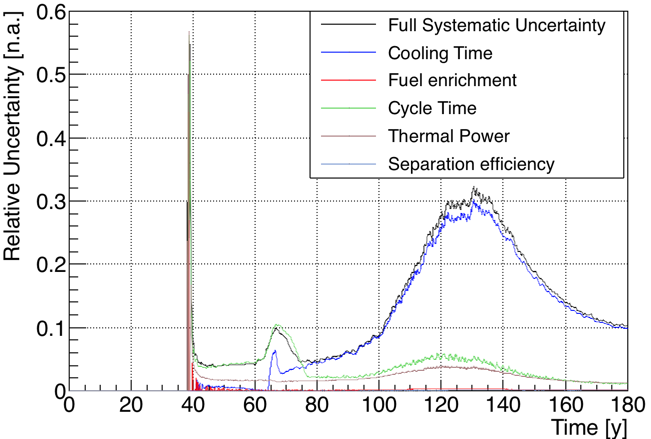
\includegraphics[scale=0.35]{pu_uncer}
    \caption{Fissile (plutonium) inventory relative uncertainty, with
    in black the total uncertainty at 1$\sigma$, and in color the uncertainty
    contribution of each parameter: cooling time (blue), fuel enrichment (red),
    cycle time (green), thermal power(brown), separation efficiency (light
    blue).}\label{fig:pu_uncer}
\end{figure}

Regarding the uncertainty, beside the low inventory artefact observable around
year 40, the relative uncertainty starts at about $5\%$, and grows until year
125 to decrease up to $10\%$ at the end of the simulation time (180y), it seems
it would have reached an equilibrium between $5$ and $10\%$ with longer
simulations...
Between year 40 and 70, the main contributor to the fissile inventory
uncertainty is the cycle length, as for the uranium needs, lower cycle length
implies more fuel loads.  Never the less, around year 65 (see Figure
\ref{fig:used_fuel}), the stock of used fuel available for reprocessing starts
to lack, and the availability of the used fuel starts to dictate the evolution
of fissile in storage.  The uncertainty weight is then slowly transferred from
the cycle length to the fuel cooling time.

\begin{figure}[ht] % replace 't' with 'b' to force it to be on the bottom
    \centering
    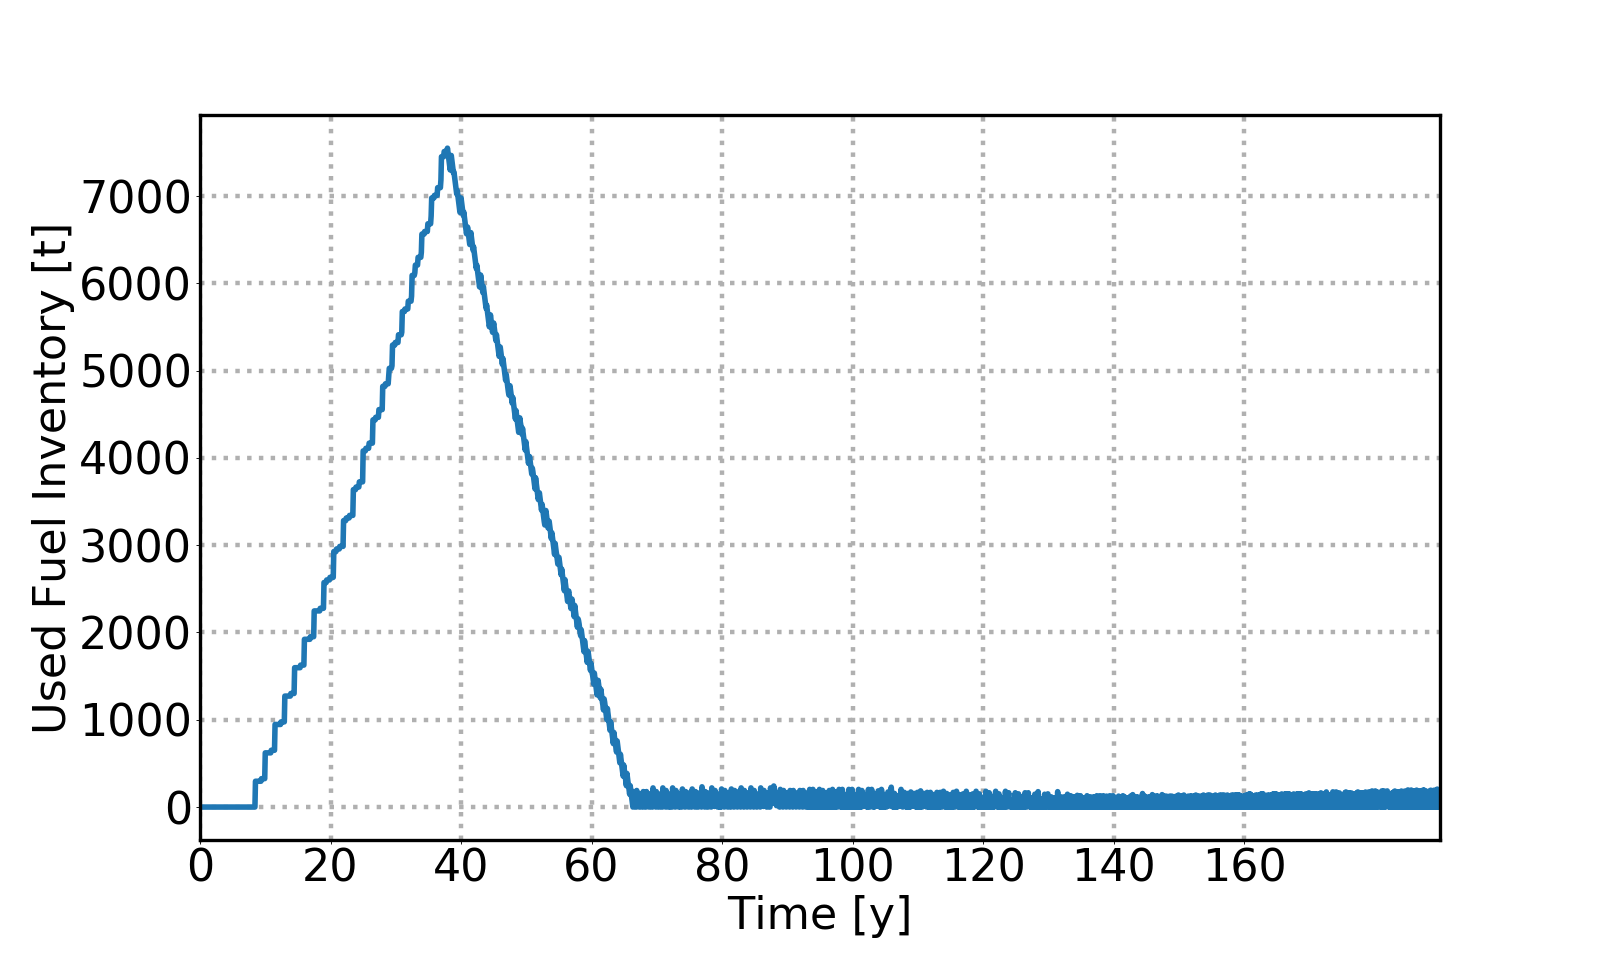
\includegraphics[scale=0.18]{used_fuel}
    \caption{Used fuel inventory.}\label{fig:used_fuel}
\end{figure}
Between year 90 and 120, the \glspl{FBR} deployment speed increases, it has to
compensate the non replacement of the decommissioned \glspl{LWR} as well as
follow the power demand.  During this period the needs in plutonium are higher
than its productions, explaining the observed decrease of the total amount, and
the increase associated relative uncertainty.

As the transition ends, the plutonium breed from the \glspl{FBR} starts to be
sufficient to sustain the new \glspl{FBR} deployment to follow the power demand.

It is also interesting to note that, the uncertainty contribution from the cycle
length is between year 40 and 70 comes mainly from fuel batch loading
frequencies, and after it relative contributions follows closely the thermal
power one, suggesting a contributions through fuel discharge burnup (i.e. fuel
discharge composition).

\subsection{Discussion}

Uranium consumption and separated fissile inventory are two important metrics
regarding to non proliferation and nuclear archaeology. In this study, we have
been able to estimate than the cycle length uncertainty of $10\%$ implies a
variation of $3\%$ to $5\%$ on the total uranium needs uncertainty, where $\approx10\%$
on the enrichment implies a almost flat uncertainty of $2\%$.

Regarding the reprocessed fissile inventory, this study has shown the limited
impact of the reprocessed fuel compositions (through burnup variations) it
limited to $5\%$, where fuel availability constrains, fuel loading frequency (cycle
time), or fissile materials available for fuel fabrication (cooling time) can lead to higher
uncertainties, respectively up to $10\%$ and to $30\%$. Moreover it is very
interesting to observe the pressure transition from one to the other around
year 70.


\section{Conclusion}

Two main points can be deduced from this work.  Firstly, in a transitional
fuel cycle, the uncertainty contributions to an output metric can vary over time
depending of various factors: deployment schedule artifact or pressure point in
the material flows.

Secondly, it is important to note the special character of the time related
parameters uncertainty in a fuel cycle study, such as cooling time and cycle
length. Where some of those time related parameter will on the first order only
impact material availability (as the cooling time will do), some other, like
cycle length, will also have a impact as physical parameters such as fuel
enrichment or thermal power. 

Cycle length impacts the discharge fuel burnup, it also affects the frequency of
the fuel loads, this, as well as the cooling may imply a uncertainty on the
material availability, which could lead to an artificially large uncertainty.
Those kind of time related uncertainties will require a careful analysis on further
uncertainty analysis, in order to understand and measure accurately their
contributions on uncertainties.

This study aims to be a proof-of-principle for uncertainty propagation in
potential commercial fuel cycle transition. While it has demonstrated the
capability to measure the uncertainty on output fuel cycle metrics and their
relative contributions, it has only been applied to systematic uncertainties per
facilities (parameters randomly generated at each new facility deployment).
This kind of study will to be extended to random uncertainty (new parameter
values at each occurrence) and completely systematic uncertainty (shared by all
the facilities of a kind).

While the parameters contributing to natural uranium needs and fissile inventory
uncertainties might be obvious, such study allows to estimate each parameters
contribution, it could be less obvious for other parameters, such as
plutonium quality, waste compositions.  Such studies could also provide research
guidance for nuclear archaeology works, which aims to precisely estimate past
fissile production by the different nuclear countries.



%%%%%%%%%%%%%%%%%%%%%%%%%%%%%%%%%%%%%%%%%%%%%%%%%%%%%%%%%%%%%%%%%%%%%%%%%%%%%%%%
%% \appendix
%% \section{Appendix}
%%
%% Numbering in the appendix is different:
%% \begin{equation} \label{eq:appendix}
%%   2 + 2 = 5\,.
%% \end{equation}
%% and another equation:
%% \begin{equation} \label{eq:appendix2}
%%   a + b = c\,.
%% \end{equation}
%%
%%%%%%%%%%%%%%%%%%%%%%%%%%%%%%%%%%%%%%%%%%%%%%%%%%%%%%%%%%%%%%%%%%%%%%%%%%%%%%%%
%% \section{Nomenclature}
%%
%% \begin{table}[H]
%%     \centering
%%     \begin{tabular}{l|l}
%% %         &  \\
%%         $N$ & Feed assay \\
%%         $N'$ & Product assay \\
%%         $N''$ & Tails assay \\
%%         $\alpha$ & Feed to product enrichment factor \\
%%         $\beta$ & Feed to tail enrichment factor \\
%%         $\theta$ & Cut
%%     \end{tabular}
%% %    \caption{Caption}
%%     \label{tab:my_label}
%% \end{table}

%% \begin{figure}[ht] % replace 't' with 'b' to force it to be on the bottom
%%   \centering
%%   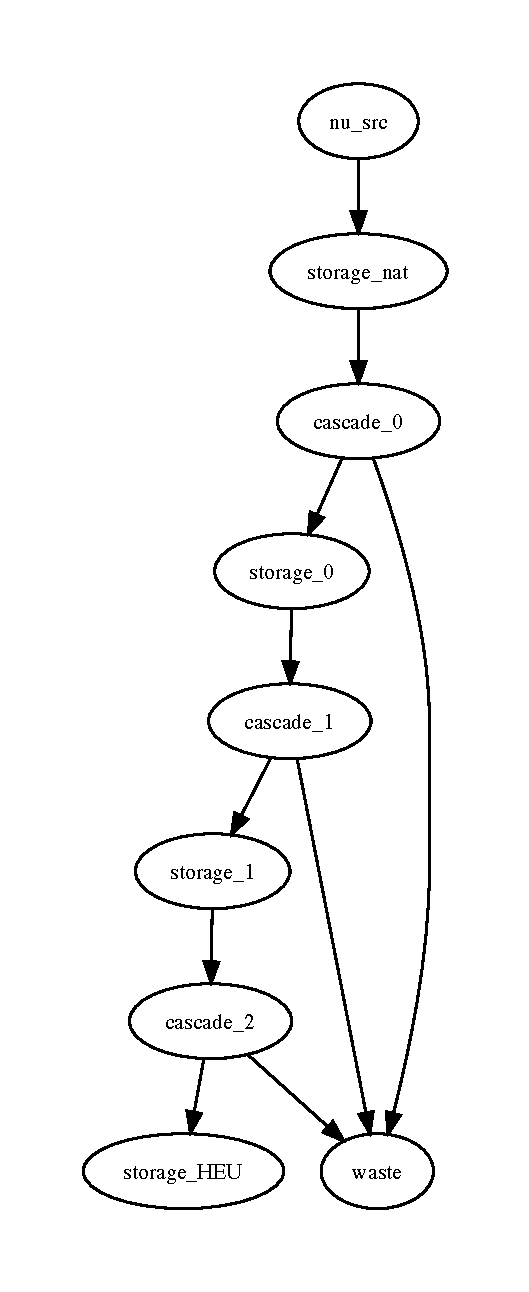
\includegraphics[scale=0.68]{flow_case_2_no_recy.pdf}
%%   \caption{Illustration of the material flow between the different level of
%%       cascades without tail recycling, in this diagram, nu\_src corresponds to
%%       an infinite source of natural uranium, cascade\_ $\{n\}$ and storage\_
%%       $\{n\}$ to the cascade and the storage getting the products of the
%%       cascades at the level $\{n\}$.}\label{fig:flow}
%% \end{figure}

%% \begin{table}[htb]
%% \centering
%%   \caption{Summary of cascade properties for each level.}
%% \begin{tabular}{cllll}
%% \toprule
%%
%% Level   &           & Assay     &       & Machines  \\
%%         & Feed      & Product   & Feed  &           \\
%% \midrule
%% 0       & 0.0071    & 0.0413    & 0.0029 & 167       \\
%% 1       & 0.0413    & 0.2043    & 0.0173 & 169       \\
%% 2       & 0.2043    & 0.5941    & 0.0971 & 168       \\
%% 3       & 0.5941    & 0.8834    & 0.3915 & 168       \\
%% 4       & 0.8834    & 0.9735    & 0.7746 & 169       \\
%%
%% \bottomrule
%% \end{tabular}
%%
%%   \label{tab:cascadelvl}
%% \end{table}

%%%%%%%%%%%%%%%%%%%%%%%%%%%%%%%%%%%%%%%%%%%%%%%%%%%%%%%%%%%%%%%%%%%%%%%%%%%%%%%%
\section{Acknowledgments}
This work was funded by the Consortium for Verification Technology under
Department of Energy National Nuclear Security Administration award number
DE-NA0002534

%%%%%%%%%%%%%%%%%%%%%%%%%%%%%%%%%%%%%%%%%%%%%%%%%%%%%%%%%%%%%%%%%%%%%%%%%%%%%%%%
\bibliographystyle{ans}
\bibliography{bibliography}
\end{document}
